\appendix
\clearpage
\addappheadtotoc
\appendixpage
\chapter{Vagrant}
\begin{figure}[!htb]
  \centering
    
\includegraphics[width=0.3\linewidth]{./img/anexos/1.png}
    \caption{Logo de Vagrant.}
  \label{fig:yo}
\end{figure}
\section{¿Qué es?}
Vagrant es una herramienta que nos ayuda a crear y manejar máquinas virtuales con un mismo entorno de trabajo. Nos permite definir los servicios a instalar así como también sus configuraciones. Está pensado para trabajar en entornos locales y lo podemos utilizar con shell-scripts, Chef, Puppet o Ansible como métodos de provisión de los recursos necesarios en la máquina virtual a desplegar.\newline
\newline
Cabe destacar que vagrant no tiene la capacidad para correr una maquina virtual por si mismo, sino que simplemente se encarga de las características con las que debe crearse esa maquina virtual y los complementos a instalar en ella o recursos de aprovisionamiento. Para poder trabajar con las máquinas virtuales es necesario que también tengamos un proveedor de maquinas virtuales, como pueden ser  VirtualBox , WMware.

\section{Instalación}

En mi caso hice uso de Vagrant sobre Windows por lo que el método de instalación era descargar un gestor de instalación de ventanas y seguir los pasos establecidos.

\begin{itemize}
    \item \url{https://www.vagrantup.com/downloads.html}
\end{itemize}
Podemos comprobar que la instalación se ha concluido satisfactoriamente haciendo uso de la shell o de la powershell. Escribimos vagrant -v debería mostrarnos la versión de vagrant actual que tenemos montada.\newline
\newline
Una vez instalado Vagrant y predispuesto el fichero Vagrantfile únicamente debemos abrir la shell, powershell en Windows. Ir al directorio en cuestión donde tenemos el fichero VagrantFile y hacer \textbf{vagrant up}. Este proceso puede tardar más o menos en función de si lo hacemos la primera vez o ya hemos hecho uso de la \textit{box} con la que se va montar la máquina virtual.

\section{¿Para que sirve?}

Como hemos venido mencionado vagrant sirve para ayudarnos a crear y configurar máquinas virtuales con determinadas características y componentes. La gran ventaja de vagrant es que posee un archivo de configuración \textbf{Vagrantfile} donde se centraliza toda la configuración de la VM que creamos además de añadir los métodos de aprovisionamiento de la maquina virtual.\newline
\newline
Esto lo puede hacer vía shell-scripts que carga en la maquina virtual a gestionar o con la API que tienen establecida dándonos la posibilidad de describir en el mismo Vagrantfile los scripts deseados. El punto positivo de Vagrant es el hecho de que se puede compartir de una forma relativamente sencilla una maquina virtual con una serie de configuraciones y recursos montados. Esto se puede hacer únicamente compartiendo el archivo de VagrantFile.

\section{¿Cómo funciona?}
Antes introdujimos el término de \textit{Box}. Vagrant cuando lee el fichero de VagrantFile lee la imagen sobre la que se va a construir la máquina virtual. Esta imagen por así llamarla, es una imagen de un SO con ciertas configuraciones ya predispuestas. Esto ahorrará tiempo en el momento de hacer el boot de la misma. Aquí puede encontrar numerosas Boxes creadas por los usuarios o por propias empresas mantenedoras de ciertos SO's.
\begin{itemize}
    \item \url{https://app.vagrantup.com/boxes/search}
\end{itemize}
\begin{figure}[!htb]
  \centering
    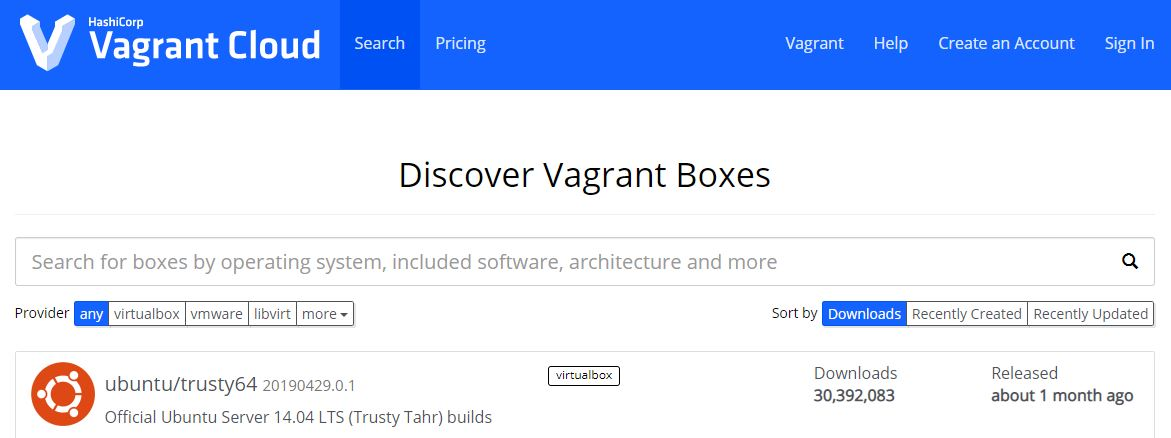
\includegraphics[width=0.7\linewidth]{./img/anexos/2.JPG}
    \caption{Repositorio de Boxes.}
  \label{fig:yo}
\end{figure}

\section{Comandos útiles}
\begin{minted}{shell}[]
# Arrancar una maquina virtual /  Parar una maquina virtual
vagrant up / vagrant halt
# Conectarse vía ssh
vagrant ssh
# Listar maquinas creadas
vagrant global-status
# Eliminar maquina 
vagrant destroy [id]
\end{minted}
\newpage
\chapter{Generar grafos desde programas p4}
\label{chap:como generar grafos desde programas p4}
\section{p4c-graphs}
Muchas veces, cuando se está programando en p4 se nos escapa el flujo de trabajo que seguirá nuestro switch. P4 al tener unas características de diseño tan modulares, permite tras un análisis sintáctico generar un diagrama de bloques ó una representación simbólica de los elementos constituidos del switch mediante un esquema gráfico. Esta \textit{feature} es un \textit{backend} del compilador \textit{p4c}, que por defecto se instala a la hora de hacer un build del compilador (Siempre y cuando las dependencias para este estén instaladas previamente).\newline
\newline
Si se tiene instalado p4c, pero no encuentra p4c-graphs, siga estos pasos:
\begin{itemize}
    \item Lo primero que vamos hacer es instalar las dependencias necesarias para poder llevar a cabo la instalación de p4c-graphs.
        \begin{itemize}
            \item \textbf{sudo apt-get install libboost-graph-dev}
        \end{itemize}
    \item Una vez las dependencias están instaladas, el proceso automático de build de p4c al volverlo a lanzar debería hacer un build de p4c-graphs.
        \begin{itemize}
            \item \textbf{cd ./testP4/tutorial\_p4/vm/p4c/build/}
            \item Preconfiguramos el build: \textbf{sudo cmake ..}
            \item Se puede acelerar el proceso de compilación, indicando número de cores que dispongamos en la máquina: \textbf{sudo make -jNUM\_CORES}
            \item Para tener un acceso global a herramienta solo quedaría: \textbf{sudo make install}.
            \item Creará softlinks, enlaces simbólicos, a los ejecutables, en la ruta \textbf{/usr/local/bin} que está en path, para ser accesible por todos.
        \end{itemize}
\end{itemize}
\section{Herramienta auto\_graph.sh}
Normalmente trabajar con p4c-graphs se hace pesado ya que nos crea muchos ficheros *.dot que debemos parsear a formato png para poder ver la figuras gráficamente. \newline
\newline
Por esto, se ha creado una herramienta que automatiza todo el proceso. Se llama auto\_graph.sh, es un shellscript que te creará un directorio llamado graph, donde podrás encontrar todos los grafos en formato png de tu programa p4. Adicionalmente, te creará un subdirectorio llamado dot, donde te almacenará también todos los ficheros *.dot generados por p4c-graphs.
\begin{itemize}
    \item Donde encontrarla: \url{https://github.com/davidcawork/testP4/blob/master/tools/auto_graph.sh}
    \item Uso: \textbf{./auto\_graph.sh [programa p4]}
\end{itemize}
\newpage
\section{Ejemplo}

\begin{minted}{c}
parser MyParser(packet_in packet, out headers hdr, inout metadata meta, 
                inout standard_metadata_t standard_metadata) {
    state start {
        transition parse_ethernet;
    }

    state parse_ethernet { 
        packet.extract(hdr.ethernet);
        transition select(hdr.ethernet.etherType) {
            TYPE_IPV4 : parse_ipv4;
	    TYPE_MYTUNNEL : parse_mytunnel;
            default : accept;
        }
    }
    
    state parse_mytunnel {
	    packet.extract(hdr.myTunnel);
	    transition select (hdr.ethernet.etherType) {
		    TYPE_IPV4 : parse_ipv4;
		    default : accept;
	    }
    }
    state parse_ipv4 {
        packet.extract(hdr.ipv4);
        transition accept;
    }
}
\end{minted}
\begin{figure}[!htb]
  \centering
    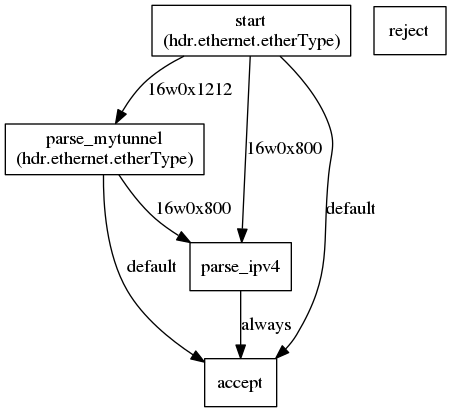
\includegraphics[width=0.6\linewidth]{./img/test/17.png}
    \caption{Bloque funcional MyParser}
  \label{fig:yo}
\end{figure}





